\documentclass{article}
\usepackage{import}
\subimport{../}{preamble}
\begin{document}

\section{Modified Method for Controllable Fabrication of Spherical AuNP Tips}

\begin{wrapfigure}{O}{0.4\textwidth}
\vspace{-10pt}
%\begin{figure}[bt]
\centering
\begin{singlespace}
\fontsize{10pt}{1em}\selectfont \subimport{./figures/}{new_setup.pdf_tex}
\end{singlespace}
\caption[Diagram of the modified method for electrochemical AuNP tip fabrication.]{\textbf{Diagram of the modified electrochemical cell for electrochemical AuNP tip fabrication.} The FTO glass active electrode used for simultaneous fabrications is removed and replaced with an aluminium clamp fitting a single tip along with the addition of a Pt reference electrode. Over potentials are now measured relative to the reference electrode.}
\label{fig:new_method}
%\end{figure}
\end{wrapfigure}

% The new method
The previous method of fabrication provided a means of demonstrating that electrodeposition can be used to produce spherical AuNP tip apices but failed to give sufficient reproducibility or understanding of growth due to the variability in the FTO working electrode contact resistance and scale with respect to the attached tips. A modified cell geometry for pulsed electrodeposition on a single tip improves upon the fabrication process. The setup, shown in \figurename~\ref{fig:new_method}, does not have the capability of simultaneously depositing on multiple tips but provides more control and monitoring of the growth of a single tip.

% Why use Pt and not Au - is it plasmonic/dielectric?
To retain good plasmonic confinement to the spherical AuNP apex, Pt-coated AFM tips are used as a base structure to maintain an electromagnetic boundary between the AuNP and the tip. Tips are cleaned prior to electrodeposition through a \SI{10}{\minute} O\subs2 plasma pretreatment. A compact potentiostat (Ivium CompactStat) replaces the larger potentiostat and a 3d-printed electrode support frame is used for stability.%
\footnote{3d-printed support frame designed and printed by Richard W. Bowman.}
Controllability is improved by measuring the deposition current more carefully with a referenced potential. The high impedance of conventional solution-based reference electrodes reduces their response time and therefore the temporal bandwidth of current measurements. Pt wire, with its large conductivity and chemical inertness, is used instead to maintain a high bandwidth during 10--\SI{100}{ms} pulsed electrodeposition \cite{sawyer1995electrochemistry}.
% Change of active electrode
The quality of the AFM probe contact with the working electrode is a highly influential factor determining the reproducibility between repeated experiments. Unreliable contacting of the tips to the FTO glass is likely the dominant reproducibility limitation in the initial setup. This is improved by replacing the FTO glass with an aluminium clamp capable of holding a single tip. Though it prevents simultaneous fabrication of multiple tips, the clamp provides a reliable, highly conductive contact to maintain a stable potential.

\begin{figure}[bt]
\centering
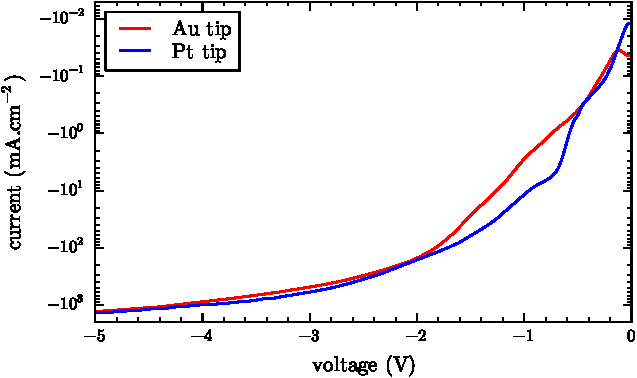
\includegraphics{figures/linear_sweep_measurements}
\caption[Linear sweep measurements of Pt and Au AFM tips in the improved electrochemical cell]{\textbf{Linear sweep measurements of Pt and Au AFM tips in the improved electrochemical cell.} More current is generated on Pt than on Au at low overpotentials, likely due to increased water splitting, though there is little difference between the two once $V\leq\SI{-2}{V}$.}
\label{fig:linear_sweeps}
\end{figure}

% Major changes
The major consequence of the electrochemical cell changes is the potential shift caused by the addition of the reference electrode. Since the working electrode potential is now relative to the solution, rather than the counter electrode, the magnitude of the potential decreases. Linear voltage sweep measurements of both Au and Pt tips (\figurename~\ref{fig:linear_sweeps}) show that the onset of growth is earlier than before at \SI{-0.6}{V}. Pt also exhibits higher currents than Au between \SI{-2}{V} and \SI{-0.6}{V}, which are attributed to Pt's catalytic properties lowering the oxidation potential of water. With respect to the fabrication procedure, the previously valid voltages of $-6$ to \SI{-8}{V} no longer produce successful growths. Reoptimisation of deposition parameters is required to ensure reliable growth.
%The result of this is that successful fabrications occur mostly around \SI{-3}{V}. Similar exposure times are still used.

%%%%%%%%%%%%%%%%%%%%%%%%%%%%
% Changes to solution
\begin{figure}[h]
\centering
\begin{subfigure}[t]{0.48\textwidth}
\caption[Diffusion-limited currents during electrodeposition for different potentials.]{\textbf{Diffusion-limited currents during electrodeposition for different potentials.}}
\label{fig:voltage_saturation_current}
\end{subfigure}
\ \
\begin{subfigure}[t]{0.48\textwidth}
\caption[Comparison of growth localisation at different potentials.]{\textbf{Comparison of growth localisation at different potentials.} The more negative the potential the more localised growth is to the apex.}
\label{fig:growth_localisation}
\end{subfigure}
\caption{Both growth localisation and current increase with more negative potentials.}
\end{figure}

As in the previous setup, the more negative the potential the more localised growth to the apex (\figurename~\ref{fig:growth_localisation}). This is particularly the case with the edge growth which becomes thicker and shorter as the voltage decreases. Short cantilevers exhibit cleaner growth to only edges and the apex compared with long cantilevers - an effect attributed to charging during plasma cleaning. To improve control whilst maintaining a larger negative potential the ECF60 solution is diluted 50\%. This lessens any concentration gradients (leading to diffusion-limited growth) and maintains drift towards the tip apex whilst providing more time to deposit the necessary amount of Au at the apex.
%%%%%%%%%%%%%%%%%%%%%%%%%%%%

\end{document}